\documentclass[11pt]{article}\title{\textbf{Practica 2}}
\author{Carmen Alonso Jimenez\\
		2º Informatica A}
\date{28/10/2022}
\addtolength{\topmargin}{-4cm}
\addtolength{\textheight}{4cm}
%\usepackage[spanish]{babel}
\usepackage[a4paper, margin=3cm, top=5mm, bottom=15mm]{geometry}
\usepackage{graphicx}
\usepackage{tikz}
\usetikzlibrary{automata, arrows.meta, positioning}

\begin{document}

\maketitle
\thispagestyle{plain}
\setlength{\parskip}{8pt}

\section{Consider the language over the alphabet {a, b} that only contains the string a. Build a DFA that recognizes this language and rejects all those strings that do not belong to the language.} 

\subsection{Mathematical description of the automaton}


	$M=(\{q_0, q_1, q_2\},\{a, b\},\delta,q_0,\{q_1\})$ with: 

$\delta = \{("q_0","a","q_1"), ("q_0","b","q_2"), ("q_1","a","q_2"),
	("q_2","a","q_2"),  ("q_2","b","q_2"), ("q_1","b","q_2")\}$

Or also $M=(\{q_0, q_1, q_2\},\{a, b\},\delta,q_0,\{q_1\})$ as a DFA with:\\

\begin{table}[h!]
\begin{tabular}{c|c|c}
  $\delta(q,\sigma)$ & $a$ & $b$\\
  \hline
  $q_0$& $q_1$ & $q_2$\\
  \hline
  $q_1$& $q_2$ & $q_2$\\
  \hline
  $q_2$& $q_2$ & $q_2$
\end{tabular}
\end{table}


\begin{center}
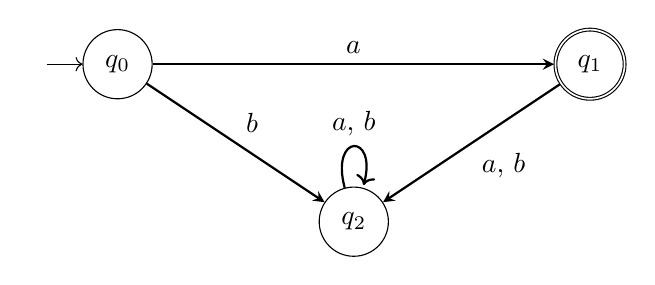
\begin{tikzpicture} [node distance = 2 cm, on grid, auto]
    \node (q0) [state, initial, initial text = {}] {$q_0$};
    %\node [state] {$q_0$};
    %\node[inner sep=0pt,outer sep=-1pt,left=0pt of q0.west]{$>$};
    \node (q1) [state, accepting] at (6,0) {$q_1$};
    \node (q2) [state] at (3,-2) {$q_2$};
    \path [-stealth, thick]
    (q0) edge node {$a$}   (q1)
    (q1) edge node {$a$, $b$}   (q2)
    (q2) edge [loop above]  node {$a$, $b$}()
    (q0) edge node {$b$} (q2);
    
\end{tikzpicture}
\end{center}

\subsection{Image from JFLAP}
	\begin{figure}[htp]
	\centering
	\includegraphics[scale=0.55]{Ejercicio1.jpg}
	\end{figure}

\newpage

\section{JSON file}

\begin{verbatim}
{
    "name" : "a",
    "representation" : {
      "K" : ["q0", "q1", "q2"],
      "A" : ["a", "b"],
      "s" : "q0",
      "F" : ["q1"],
      "t" : [["q0", "a", "q1"],
             ["q0", "b", "q2"],
             ["q1", "a", "q2"],
             ["q2", "a", "q2"],
             ["q2", "b", "q2"],
             ["q1", "b", "q2"]]
      }
  }

\end{verbatim}


\end{document}